\documentclass{bioinfo}
\copyrightyear{2012}
\pubyear{2012}

\usepackage{url}
%\usepackage{subfigure}
\usepackage{natbib}
\newcommand{\prog}{{\sc Ngsane}}
\newcommand{\ecoli}{{\it E.coli}}

\begin{document}
\firstpage{1}

\title[NGSANE]{Lightweight Production Informatics}
\author[Fabian A. Buske {\em et al.}]{Fabian A. Buske\,$^{1}$,
Hugh French\,$^{1}$,
Martin Smith\,$^{1}$,
and  Denis C. Bauer\,$^{1}$\footnote{Contact: \href{Denis.Bauer@CSIRO.au}{Denis.Bauer@CSIRO.au}}}
\address{
          $^{1}$Epigenetics Program, Cancer Research Division, Garvan Institute of Medical Research, Kinghorn Cancer Centre, Darlinghurst City, NSW 2010, Australia,\\
          $^{2}$Division of Computational Informatics, CSIRO, Sydney, NSW. 2113 Australia,\\
          }

\history{Received on XXXXX; revised on XXXXX; accepted on XXXXX}

\editor{Associate Editor: XXXXXXX}

\maketitle


\begin{abstract}
\section{Summary: The initial steps in sequencing data analysis can be automated. However, the individual components depreciate rapidly due to evolving technology and analysis methodology, making the whole production informatics pipeline disposable.
Hence, constructing pipelines from primary Linux commands enables the use of "hot-swappable" components compared to the stable more rigid program-call wrapping by higher level languages as used in other published pipelining systems.
Here we present \prog , a Linux-based, HPC-enabled framework that minimizes overhead for set-up and processing of new projects yet maintains full flexibility of custom scripting when processing raw sequence data.}
\section{Availability and Implementation:  \prog\ is implemented in BASH and available via GitHub 
 \url{https://github.com/allPowerde/ngsane}}
\section{Contact:} \href{Denis.Bauer@CSIRO.au}{Denis.Bauer@CSIRO.au}
\end{abstract}

\section{Introduction}

The first steps of analysing sequencing data (2GS,NGS) have entered a transitional period where analysis steps can be automated in standardised pipelines, yet due to constantly evolving technology and new application areas, maintaining these "Production Informatics" pipelines can be labour intensive. 
To address this problem several pipelining methodologies have been published in recent years with enthusiastic statements about the ease of use, some of them commercially fuelled (see a detailed list in the Supplementary). 
Other than reducing the overhead of setting up similar analysis tasks, pipeline tools aim to make research steps reproducible and document provenance. 

Many GUI-enabled tools, like Galaxy~\cite{Goecks2010}, address both aims but are commonly tailored to cater for biologist with only small numbers of experiments. 
With further decreasing sequencing costs and a higher demand on replicates to assess technical and biological variability~\cite{Auer2010}, study sizes will substantially increase making the capability of leveraging high performance compute clusters paramount. 
Catering for these demands are heavy-weight frameworks written in user-friendly languages like python ({\sc snakemake}~Koester2012, {\sc nestly}~\cite{McCoy2013}), c++ ({\sc Genomictools}~\cite{Tsirigos2012}) or Groovy ({\sc Bpipe}~\cite{Sadedin2012}). 

However, utilising an additional program language for the job submission wrapper causes the developer to be two steps removed from the actual program call. 
Hence, being able to construct pipelines from call statements that can be tested on the command line directly without syntax alterations or wrapper-script involvment provides a substantial advantage in this fast pace environment where analysis pipelines are disposable as new algorithms are developed.    
 
\prog\ is a lightweight, Linux-based, HPC-enabled framework that minimizes overhead for set-up and processing of new projects yet maintains full flexibility of custom scripting when processing raw sequence data.
Below we describe \prog's aims.

\begin{figure*}[tbh]
    \centering
   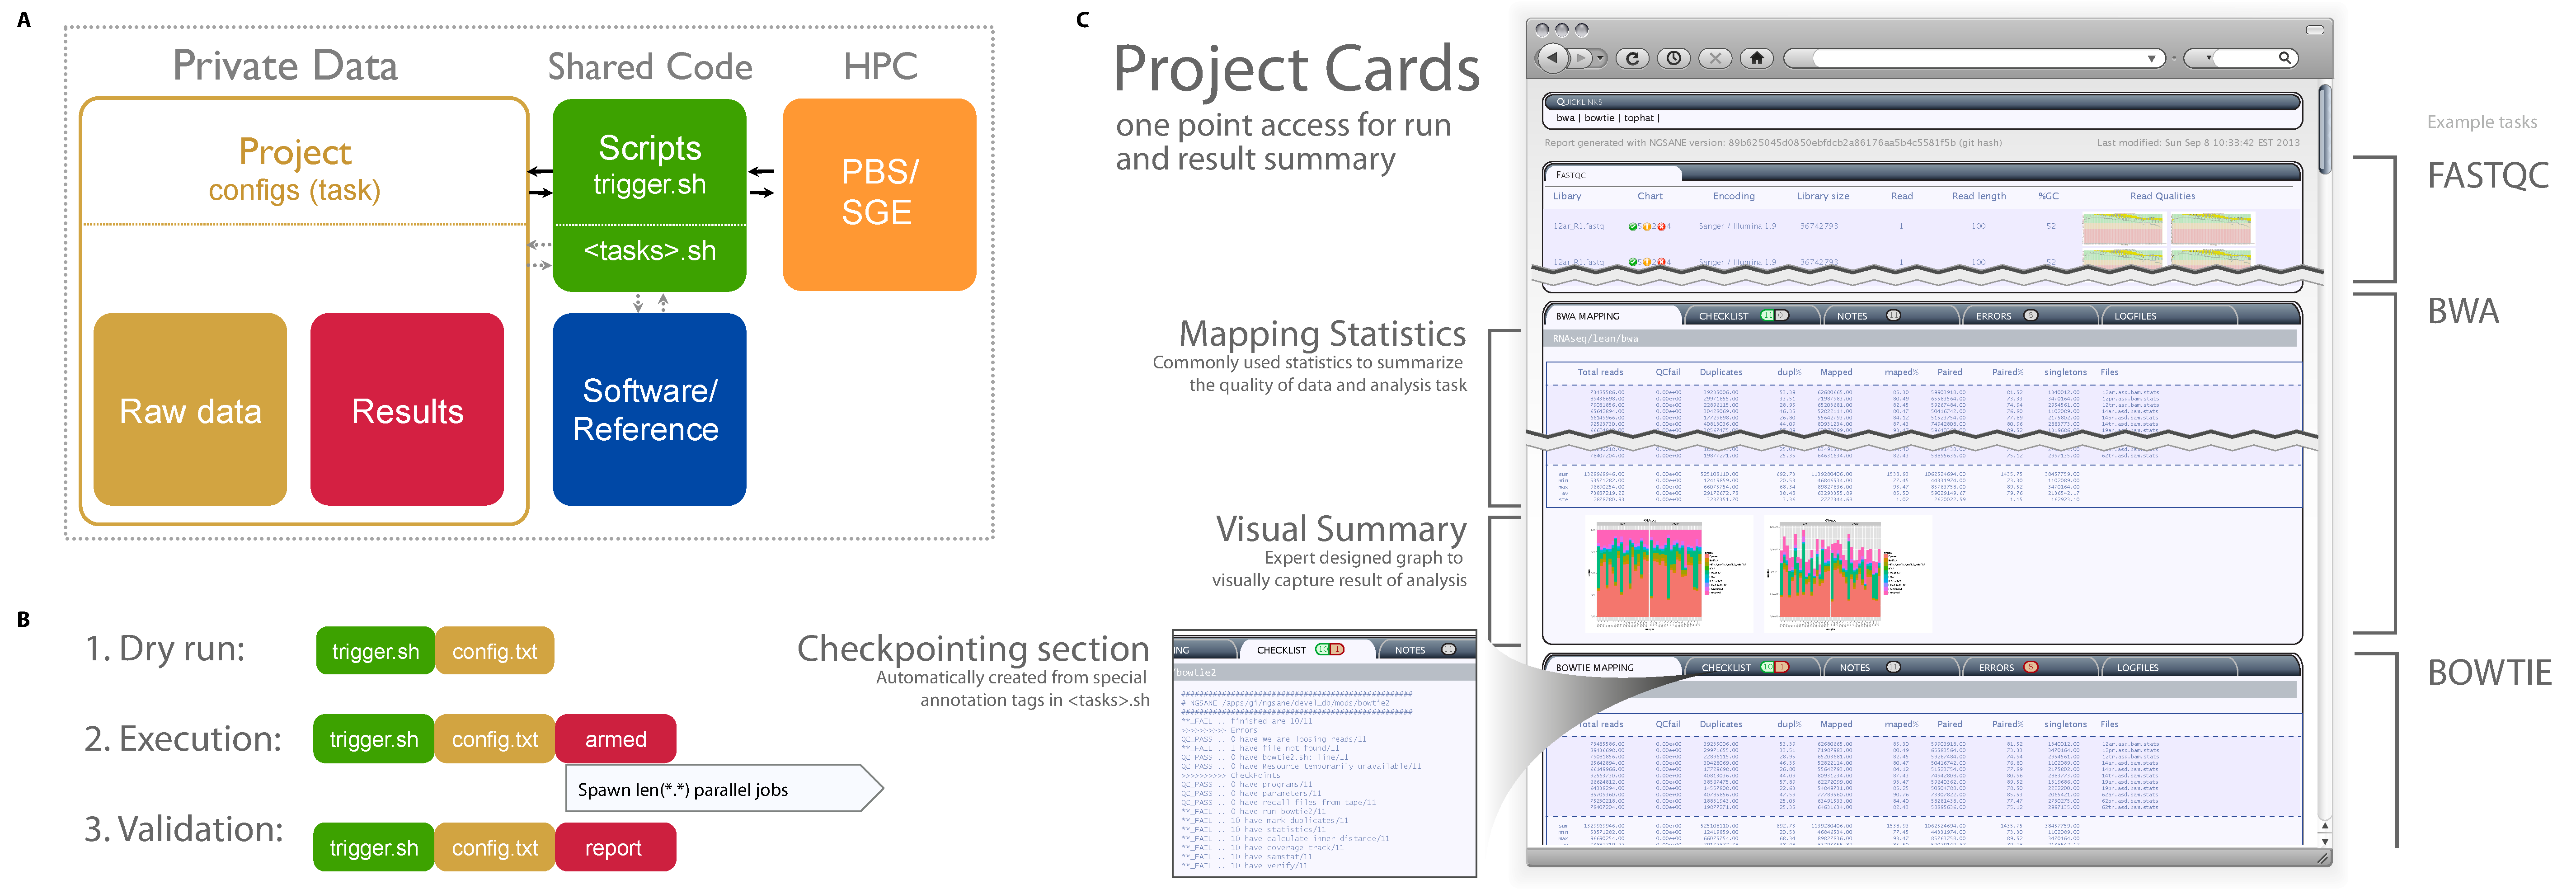
\includegraphics[type=pdf,ext=.pdf,read=.pdf, scale=0.18]{images/web_screens}
    \caption{
      {\bf Overview of \prog .} {\bf a)} Separation of software, references, scripts from project data.  {\bf b)} Workflow of \prog . {\bf c)} Resulting "project card" providing efficient visual quality control and an access point for collaborators.} 
      \label{fig:overview}
\end{figure*}

{\it Data security and reusability.}
The framework separates project specific data from reference-files, scripts, and software suites that are reusable in other projects. 
This ensures consistency while encapsulating projects and managing permissions. 
The transaction between projects and framework is facilitated by a project-specific config file defining reference data paths and which analysis to perform. 
\prog\ supports system with Hierarchical storage management, specifically Data Migration Facility (DMF), by ensuring files are online before attempting program calls. 

{\it Hot swapping and adaptability.}
Similar to the toolshed-concept in {\sc Galaxy}, individual tasks, like read mapping with a specific program, can be packaged in individual bash script modules.
Each module receives the input file (e.g. *.fastq,*.bam) via command line and can hence be executed directly on individual files during development and testing.
During production, \prog\ automatically submits separate module calls for each input file. 
This allows to swap modules in and out with no disruption to the overall system (hot swapping) and hence not slow down software incorporation (needing GUI parameter definitions, customized wrappers, language-specific overhead).

{\it High performance compute (HPC) and parallel execution.} 
\prog\ supports Sun-Grid-Engine (SGE) and Portable-Batch-System (PBS) job scheduling and can be operated in different modes for development and production thus enabling efficient and flexible processing of NGS data. 
Since this traditional HPC job partitioning and submission is modular from the program calls, the engine can be updated to utilize other architectures, e.g. hadoop. 

{\it Reproducibility and checkpoint recovery.}
A full audit trail is generated recoding performed tasks, reference data information, timestamps, software version as well as HPC log files. 
\prog\ gracefully recovers from unsuccessfully executed jobs be it due to failed commands, missing input, oder under-resourced HPC jobs by cleanly
restarting from the point of failure. 
Note, \prog\ does not utilize {\sc GNU Makefile} because {\it a)} {\sc Makefile} violates \prog 's no-syntax-alteration policy by having reserved variables making it necessary to encapsulate certain commands (e.g. {\sc awk}), and {\it b)} as noted by {\sc snakemake}, make allows only one output file per rule.   

{\it Robust execution and full monitoring.}
In contrast to {\sc Galaxy}, {\sc snakemake}, or {\sc Bpipe}, \prog\ does not focus on automated pipeline construction. 
In our experience, stages are executed sequentially with interjacent human quality scrutiny. 
\prog\ hence focuses on robust checkpointing and report generation to make stage control efficient. 
However, automated staging can be achieved by leveraging the customisable interfaces between modules and control over the HPC-queuing system from the project's config file.

{\it Automated project "summary card" creation.}
\prog\ generates a high level summary html file (project card, see Figure~\ref{fig:overview}) to enable informed decisions about the experimental success. 
This page provide an access point for new lab members or collaborators.

{\it Complete customisation.}
In addition to the project specific config file, \prog\ has a system wide config file containing details about the submission system, typical resources consumed on the platform and path or module name for the third-party analysis software.
However, \prog\ credo is that every parameter can be overwritten from the config file, hence the default parameters can be adjusted to, e.g. use a project specific software versions, request more resources, or change the output folder name. 
Additional parameters, e.g. special queue, or new parameter in a software release, can be provided to each program via a special variable in the config file, which is by default empty.  

{\it Repeat calls}
As stated by {\sc nestly}, pipelines have to be rerun on the full or a subset of the data with altered parameter settings. 
\prog\ facilitates and documents this by allowing multiple config files for each variation tested. 
Furthermore, executing \prog\ in the dry run mode will create the list of files \prog\ will submit jobs for, which can then be manually curated to submit only a subset.

{\it Knowledge transfer.}
\prog\ provides a unified framework (e.g. common folder structure ) for processing of raw data obtained from different experimental protocols. 
This helps lab members to easily understand their colleague's work and continue the workflow in a collaboration or after a handover. 


%\begin{methods}
%\end{methods}
%\section{Results}

\prog\ can be forked via GitHub allowing monitored contribution from collaborators. 
It currently includes pipelines for adapter trimming, read mapping, peak calling, motif discovery, transcript assembly, variant calling and chromatin conformation analysis by utilising software tools currently considered as the standard. 

\subsection*{Acknowledgement}
The authors would like to thank the Queensland Brain Institute for initial and CSIRO's Transformational Capability Platform for ongoing funding.  

%\subsection*{Author contribution}

\subsection*{Competing financial interests}
None declared

\bibliographystyle{natbib}
\bibliography{ngsane}

\end{document}
